\documentclass[12pt]{article}

\usepackage{TLR}

\usepackage{graphicx,url}

\usepackage[brazil]{babel}   
%\usepackage[latin1]{inputenc}  
\usepackage[utf8]{inputenc}  
% UTF-8 encoding is recommended by ShareLaTex

     
\sloppy
\title{Técnica para levantamento de requisitos}
\author{Rodrigo Visentainer}
\address{Sistemas de Informação -- Universidade Católica de Santa Catarina}
\begin{document} 
\maketitle
\begin{resumo} 
  As técnicas de levantamento de requisitos têm por objetivo superar as dificuldades relativas a esta fase. Todas as técnicas possuem um conceito próprio e suas respectivas vantagens e desvantagens, que podem ser utilizadas em conjunto pelo analista. Serão apresentadas de forma resumida nesse artigo algumas técnicas de levantamento de requisitos.
\end{resumo}
\section{Introdução}
Sommerville (2003) propõe um processo genérico de levantamento e análise que contém as seguintes atividades:
\begin{itemize}
\item Compreensão do domínio: Os analistas devem desenvolver sua compreensão do domínio da aplicação;
\item Coleta de requisitos: É o processo de interagir com os stakeholders do sistema para descobrir seus requisitos. A compreensão do domínio se desenvolve mais durante essa atividade;
\item Classificação: Essa atividade considera o conjunto não estruturado dos requisitos e os organiza em grupos coerentes;
\item Resolução de conflitos: Quando múltiplos stakeholders estão envolvidos, os requisitos apresentarão conflitos. Essa atividade tem por objetivo solucionar esses conflitos;
\item Definição das prioridades: Em qualquer conjunto de requisitos, alguns serão mais importantes do que outros. Esse estágio envolve interação com os stakeholders para a definição dos requisitos mais importantes;
\item Verificação de requisitos: Os requisitos são verificados para descobrir se estão completos e consistentes e se estão em concordância com o que os stakeholders desejam do sistema.
O levantamento e análise de requisitos é um processo iterativo, com uma contínua validação de uma atividade para outra, conforme exemplificado pela Figura 1.
\end{itemize}

\begin{figure}[ht]
\centering
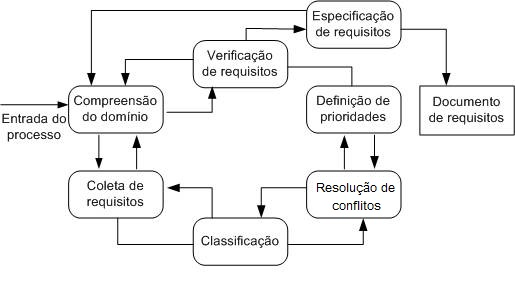
\includegraphics[width=.9\textwidth]{IMG-1.jpg}
\caption{Processo interativo}
\label{fig:scrumboard}
\end{figure}

\pagebreak

\section{Dificuldades encontradas}
Entre as dificuldades encontradas na fase de levantamento de requisitos estão: o usuário principal do sistema não sabe o que quer que o sistema faça ou sabe e não consegue transmitir para o analista; requisitos identificados, mas que não são realistas e não identificam os requisitos similares informados por pessoas diferentes. Um stakeholder errado afetará em perda de tempo e dinheiro para ambas as partes envolvidas no desenvolvimento do sistema.

Identifica-se um levantamento de requisitos adequado através da boa definição do projeto, da efetividade do projeto, de informações necessárias a um perfeito diagnóstico e de soluções inteligentes. Quanto ao levantamento de requisitos inadequado, o resultado é um diagnóstico pobre com conclusões comprometidas, não identificação das causas dos problemas, custos elevados, prazos vencidos ou comprometedores, omissão de processos fundamentais e descréditos.

\section{Entrevistas}

A entrevista é uma das técnicas tradicionais mais simples de utilizar e que produz bons resultados na fase inicial de obtenção de dados. Convém que o entrevistador dê margem ao entrevistado para expor as suas idéias. É necessário ter um plano de entrevista para que não haja dispersão do assunto principal e a entrevista fique longa, deixando o entrevistado cansado e não produzindo bons resultados.

As seguintes diretrizes podem ser de grande auxílio na direção de entrevistas bem sucedidas com o usuário: desenvolver um plano geral de entrevistas, certificar-se da autorização para falar com os usuários, planejar a entrevista para fazer uso eficiente do tempo, utilizar ferramentas automatizadas que sejam adequadas, tentar descobrir que informação o usuário está mais interessado e usar um estilo adequado ao entrevistar.

Para planejar a entrevista é necessário que antes dela sejam coletados e estudados todos os dados pertinentes à discussão, como formulários, relatórios, documentos e outros. Dessa forma, o analista estará bem contextualizado e terá mais produtividade nos assuntos a serem discutidos na entrevista.

É importante determinar um escopo relativamente limitado, focalizando uma pequena parte do sistema para que a reunião não se estenda por mais de uma hora. O usuário tem dificuldade de concentração em reuniões muito longas, por isso é importante focalizar a reunião no escopo definido.

Após a entrevista é necessário validar se o que foi documentado pelo analista está de acordo com a necessidade do usuário, que o usuário não mudou de opinião e que o usuário entende a notação ou representação gráfica de suas informações.

\section{Questionários}

O uso de questionário é indicado, por exemplo, quando há diversos grupos de usuários que podem estar em diversos locais diferentes do país. Neste caso, elaboram-se pesquisas específicas de acompanhamento com usuários selecionados, que a contribuição em potencial pareça mais importante, pois não seria prático entrevistar todas as pessoas em todos os locais.

Existem vários tipos de questionários que podem ser utilizados. Entre estes podemos listar: múltipla escolha, lista de verificação e questões com espaços em branco. O questionário deve ser desenvolvido de forma a minimizar o tempo gasto em sua resposta.

Na fase de preparação do questionário deve ser indicado o tipo de informação que se deseja obter. Assim que os requisitos forem definidos o analista deve elaborar o questionário com questões de forma simples, clara e concisa, deixar espaço suficiente para as repostas que forem descritivas e agrupar as questões de tópicos específicos em um conjunto com um título especial. O questionário deve ser acompanhado por uma carta explicativa, redigida por um alto executivo, para enfatizar a importância dessa pesquisa para a organização.

Deve ser desenvolvido um controle que identifique todas as pessoas que receberão os questionários. A distribuição deve ocorrer junto com instruções detalhadas sobre como preenchê-lo e ser indicado claramente o prazo para devolução do questionário. Ao analisar as respostas dos participantes é feito uma consolidação das informações fornecidas no questionário, documentando as principais descobertas e enviando uma cópia com estas informações para o participante como forma de consideração pelo tempo dedicado a pesquisa.

\section{Conclusão}

Não existe uma técnica padrão para o processo de levantamento de requisitos. Para alcançar um levantamento de requisitos mais preciso é importante o conhecimento de diversas técnicas para saber que técnica de levantamento aplicar em cada situação.

É primordial que o analista possua perfil adequado. O analista de sistemas precisa de mais do que apenas a capacidade de desenhar fluxogramas e outros diagramas técnicos. O analista de sistemas tem a função de projetar e analisar sistemas de ótimo desempenho. Para que esse objetivo seja alcançado, é necessário o analista de sistema possuir a capacidade de interpretar todo o sistema.



\bibliographystyle{sbc}
\bibliography{sbc-template}


\end{document}